\chapter{От малых городов до городов-миллионеров}
\label{ch:city}

Глава посвящена исследованию различных типов городов, соответствующих четырем объектам Викиданных — <<малый город>>, <<город>>, <<большой город>> и <<города-миллионеры>>. В ходе исследования с использованием SPARQL-запросов получены данные о количестве экземпляров исследуемых объектов, а также рассмотрены вопросы, связанные со свойствами population (численность населения) и sister city (город-побратим) этих объектов Викиданных. В том числе решены следующие задачи: подсчет и анализ численности населения разных типов городов; определение числа городов, не имеющих побратимов; построение списка городов, упорядоченных по числу побратимов; нахождение числа городов с определённым числом побратимов; определение страны с наибольшим числом побратимов; нахождение ближайших соседей России. В заключении главы дана оценка полноты данных, представленных в Википедии и Викиданных, и перечислены проблемы и сложности, возникшие при изучении разных типов городов в этих проектах.
%%%%%%%%%%%%%%%%%%%%%%%%%%%%%%%%%%%%%%%%%%%%%%%%%%%%%%%
\section{Экземпляры}

Ниже представлены SPARQL-запросы для нахождения экземпляров исследуемых объектов: 
\begin{itemize}
	\item <<малый город>> или \wdqName{town}{3957}, листинг~\ref{lst:town};
	\item <<город>> или \wdqName{city}{515}, листинг~\ref{lst:city};
	\item <<большой город>> или \wdqName{big city}{1549591}, листинг~\ref{lst:big_city};
	\item <<города-миллионеры>> или \wdqName{city with millions of inhabitants}{1637706}, листинг~\ref{lst:city_million}.
\end{itemize}

Дополнительно составлен запрос для нахождения списка экземпляров объектов разных типов городов (листинг~\ref{lst:different_city_types}).

\begin{lstlisting}[ language=SPARQL, 
                    caption={\href{https://w.wiki/jfn}{Экземпляры объекта <<малый город>>}\protect\footnotemark},
                    label=lst:town, 
                    escapebegin=ку,escapeend=ку-ку>
                    ]
SELECT ?city ?cityLabel WHERE {
	?city wdt:P31 wd:Q3957. # instances of "town"
	SERVICE wikibase:label { bd:serviceParam wikibase:language "ru" }
}
\end{lstlisting}
\footnotetext{Получено \num{13800} <<малых городов>> в 2020 году. Ссылка на SPARQL-запрос: \href{https://w.wiki/jfn}{https://w.wiki/jfn}}

\marginnote[0.0cm]{Среди отечественных <<городов>> в Викиданных больше всего свойств по данным \href{https://prowd.id/dashboards/fa0470eaf5f5/profile}{ProWD}\cite{city_prowd} у \wdqName{Новороссийска}{15760} (31 свойство). Лидером по <<городам>> всего мира является \wdqName{Сингапур}{334} (104 свойства).}

\begin{lstlisting}[ language=SPARQL, 
                    caption={\href{https://w.wiki/jft}{Экземпляры объекта <<город>>}\protect\footnotemark},
                    label=lst:city, 
                    escapebegin=ку,escapeend=ку-ку>
                    ]
SELECT ?city ?cityLabel WHERE {
	?city wdt:P31 wd:Q515. # instances of "city"
	SERVICE wikibase:label { bd:serviceParam wikibase:language "ru" }
}
\end{lstlisting}
\footnotetext{Получено \num{20800} <<городов>> в 2017 году, \num{9260} <<городов>> в 2020 году. Ссылка на SPARQL-запрос: \href{https://w.wiki/jft}{https://w.wiki/jft}}

\marginnote[0.0cm]{Среди отечественных <<больших городов>> в Викиданных больше всего свойств по данным \href{https://prowd.id/dashboards/bd326207c820/profile}{ProWD}\cite{big_city_prowd} у \wdqName{Москвы}{649}  (76 свойств). Лидером по <<большим городам>> всего мира является \wdqName{Сингапур}{334} (104 свойства).}

\begin{lstlisting}[ language=SPARQL, 
                    caption={\href{https://w.wiki/jfu}{Экземпляры объекта <<большой город>>}\protect\footnotemark},
                    label=lst:big_city, 
                    escapebegin=ку,escapeend=ку-ку>
                    ]
SELECT ?city ?cityLabel WHERE {
	?city wdt:P31 wd:Q1549591. # instances of "big city"    
	SERVICE wikibase:label { bd:serviceParam wikibase:language "ru" }
}
\end{lstlisting}
\footnotetext{Получено 198 <<больших городов>> в 2017 году, \num{3075} <<больших городов>> в 2020 году. Ссылка на SPARQL-запрос: \href{https://w.wiki/jfu}{https://w.wiki/jfu}}

\begin{lstlisting}[ language=SPARQL, 
                    caption={\href{https://w.wiki/jfx}{Экземпляры объекта <<города-миллионеры>>}\protect\footnotemark},
                    label=lst:city_million, 
                    escapebegin=ку,escapeend=ку-ку>
                    ]
SELECT ?city ?cityLabel WHERE {
	?city wdt:P31 wd:Q1637706. # instances of "city 1000000+" 
	SERVICE wikibase:label { bd:serviceParam wikibase:language "ru" }
}
\end{lstlisting}
\footnotetext{Получено 616 <<городов-миллионеров>> в 2020 году. Ссылка на SPARQL-запрос: \href{https://w.wiki/jfx}{https://w.wiki/jfx}}

\begin{lstlisting}[ language=SPARQL, 
                    caption={\href{https://w.wiki/jfy}{Экземпляры объектов разных типов городов}\protect\footnotemark},
                    label=lst:different_city_types, 
                    escapebegin=ку,escapeend=ку-ку>
                    ]
SELECT ?city ?cityLabel WHERE { # Selecting items which are ...
	{ ?city wdt:P31 wd:Q3957 } UNION # instances of "town"
	{ ?city wdt:P31 wd:Q515 } UNION # instances of "city"
	{ ?city wdt:P31 wd:Q1549591 } UNION # instances of "big city"
	{ ?city wdt:P31 wd:Q1637706 } # instances of "city 1000000+"                                
	SERVICE wikibase:label { bd:serviceParam wikibase:language "ru". }
}
\end{lstlisting}
\footnotetext{Получен \num{26751} экземпляр объектов разных типов городов в 2020 году.Ссылка на SPARQL-запрос: \href{https://w.wiki/jfy}{https://w.wiki/jfy}}


%%%%%%%%%%%%%%%%%%%%%%%%%%%%%%%%%%%%%%%%%%%%%%%%%%%%%%%
\section{Численность населения}

Ниже представлены SPARQL-запросы для нахождения суммарной численности населения экземпляров каждого из исследуемых объектов: 
\begin{itemize}
	\item <<малый город>> или \wdqName{town}{3957}, листинг~\ref{lst:population_town};
	\item <<город>> или \wdqName{city}{515}, листинг~\ref{lst:population_city};
	\item <<большой город>> или \wdqName{big city}{1549591}, листинг~\ref{lst:population_big_city};
	\item <<города-миллионеры>> или \wdqName{city with millions of inhabitants}{1637706}, листинг~\ref{lst:population_city_millions}.
\end{itemize}

%%%%%%%%%%%%%%%% Упражнение 1 %%%%%%%%%%%%%%%% 
\marginnote{
Какие города были названы в честь географических объектов?
\begin{itemize}
\item \href{https://bit.ly/3pgtcUs}{Тольятти}
\item \href{https://bit.ly/3eJmEsk}{Тула}
\item \href{https://bit.ly/3pa3uAV}{Черняховск}
\item \href{https://bit.ly/3eMDOp8}{Курильск}
\item \href{https://bit.ly/3kccAJC}{Вологда}
\item \href{https://bit.ly/3pfe1KW}{Обнинск}
\end{itemize}
См. ответ~\ref{answer:cities_geographic_objects} на с.~\pageref{answer:cities_geographic_objects}.
}

\begin{lstlisting}[ language=SPARQL, 
                    caption={\href{https://w.wiki/jgX}{Численность населения <<малых городов>>}\protect\footnotemark},
                    label=lst:population_town, 
                    escapebegin=ку,escapeend=ку-ку>
                    ]
# Selecting total population of items which are ...
SELECT (SUM(?population_city) as ?sum) WHERE {                    
	SELECT (MAX(xsd:integer(REPLACE(STR(?population),"\\.",""))) 
						as ?population_city) ?city WHERE {
		?city wdt:P31 wd:Q3957.	# instances of "town"
		?city wdt:P1082 ?population # with filled property "population"                                  
	}
	GROUP BY ?city
}
\end{lstlisting}
\footnotetext{Ссылка на SPARQL-запрос: \href{https://w.wiki/jgX}{https://w.wiki/jgX}}

\begin{lstlisting}[ language=SPARQL, 
                    caption={\href{https://w.wiki/jgY}{Численность населения <<городов>>}\protect\footnotemark},
                    label=lst:population_city, 
                    escapebegin=ку,escapeend=ку-ку>
                    ]
# Selecting total population of items which are ...
SELECT (SUM(?population_city) as ?sum) WHERE {                    
	SELECT (MAX(xsd:integer(REPLACE(STR(?population),"\\.",""))) 
						as ?population_city) ?city WHERE {
		?city wdt:P31 wd:Q515. # instances of "city"
		?city wdt:P1082 ?population # with filled property "population"
	}
	GROUP BY ?city
}\end{lstlisting}
\footnotetext{Ссылка на SPARQL-запрос: \href{https://w.wiki/jgY}{https://w.wiki/jgY}}

\begin{lstlisting}[ language=SPARQL, 
                    caption={\href{https://w.wiki/jga}{Численность населения <<больших городов>>}\protect\footnotemark},
                    label=lst:population_big_city, 
                    escapebegin=ку,escapeend=ку-ку>
                    ]
# Selecting total population of items which are ...
SELECT (SUM(?population_city) as ?sum) WHERE {                    
	SELECT (MAX(xsd:integer(REPLACE(STR(?population),"\\.",""))) 
						as ?population_city) ?city WHERE {
		?city wdt:P31 wd:Q1549591. # instances of "big city"
		?city wdt:P1082 ?population # with filled property "population"
	}
	GROUP BY ?city
}
\end{lstlisting}
\footnotetext{Ссылка на SPARQL-запрос: \href{https://w.wiki/jga}{https://w.wiki/jga}}

\begin{lstlisting}[ language=SPARQL, 
                    caption={\href{https://w.wiki/jgb}{Численность населения <<городов-миллионеров>>}\protect\footnotemark},
                    label=lst:population_city_millions, 
                    escapebegin=ку,escapeend=ку-ку>
                    ]
# Selecting total population of items which are ...
SELECT (SUM(?population_city) as ?sum) WHERE {
	SELECT (MAX(xsd:integer(REPLACE(STR(?population),"\\.",""))) 
						as ?population_city) ?city WHERE {
		?city wdt:P31 wd:Q1637706. # instances of "city 1000000+"
		?city wdt:P1082 ?population # with filled property "population"
	}
	GROUP BY ?city
}
\end{lstlisting}
\footnotetext{Ссылка на SPARQL-запрос: \href{https://w.wiki/jgb}{https://w.wiki/jgb}}

В разных странах используются различные символы в качестве разделителей разрядов, например, точка, запятая или пробел. Как результат, варианты представления значения свойства \href{https://www.wikidata.org/wiki/Property:P1082}{population} также могут быть различны. Проблемы возникают при использовании точки, поскольку в Викиданных этот символ является разделителем целой и десятичной частей числа. Для устранения неоднозначности необходимо использовать функцию \href{https://en.wikibooks.org/wiki/SPARQL/Expressions\_and\_Functions\#REPLACE}{REPLACE}, позволяющую удалить указанный символ (листинги \ref{lst:population_town}, \ref{lst:population_city}, \ref{lst:population_big_city}, \ref{lst:population_city_millions}). Данное преобразование не влияет на само значение, так как численность населения априори является целым числом, а разделители разрядов используются исключительно для упрощения чтения.

В таблице~\ref{tab:population} приведена сводная информация о численности населения разных типов городов, а также рассчитана доля населения, приходящегося на каждый тип города, от общего \href{https://bit.ly/3pgnMss}{населения Земли}, достигшего примерно \href{https://www.gazeta.ru/science/2020/07/16\_a\_13154515.shtml}{\num{7,8} млрд человек на 2020 год}\cite{world_population}.

\begin{table}[b]
  \centering
  \fontfamily{ppl}\selectfont
  \begin{tabular}{| l | r | r |}
    \toprule
   \multicolumn{1}{| c |}{Тип города} & \multicolumn{1}{p{0.32\textwidth} |}{\centering Численность населения (млн чел.)} & \multicolumn{1}{p{0.25\textwidth} |}{\centering \% от общего населения Земли} \\
    \midrule
    <<малый город>> & \num{53,30} & \num{0,7}\% \\
    <<город>> & \num{1133,56} & \num{14,5}\% \\
    <<большой город>> & \num{2538,49} & \num{32,5}\% \\
    <<города-миллионеры>> & \num{2118,39} & \num{27,1}\% \\
    \midrule
    \multicolumn{1}{| c |}{Всего} & \num{5843,74} & \num{74,8}\% \\
    \bottomrule
  \end{tabular}
  \caption{Численность населения разных типов городов, 2020 год.}
  \label{tab:population}
  %\zsavepos{pos:normaltab}
\end{table}



%%%%%%%%%%%%%%%%%%%%%%%%%%%%%%%%%%%%%%%%%%%%%%%%%%%%%%%
\section{Города-побратимы}

\subsection{Сколько городов обходятся без городов-побратимов?}

Ниже представлен SPARQL-запрос для нахождения числа городов, не имеющих побратимов (листинг \ref{lst:without_sister_cities}).

%\newpage % Fix: Остается одна строчка от листинга на странице

\begin{lstlisting}[ language=SPARQL, 
                    caption={\href{https://w.wiki/jgv}{Количество городов, не имеющих побратимов}\protect\footnotemark},
                    label=lst:without_sister_cities, 
                    escapebegin=ку,escapeend=ку-ку>
                    ]
# Counting items which are ... 
SELECT (COUNT(?city) as ?count) WHERE {                             
	{ ?city wdt:P31 wd:Q3957 } UNION # instances of "town"          
	{ ?city wdt:P31 wd:Q515 } UNION # OR instances of "city"                 
	{ ?city wdt:P31 wd:Q1549591 } UNION # OR instances of "big city"                       
	{ ?city wdt:P31 wd:Q1637706 } 	# OR instances of "city 1000000+"              
	FILTER NOT EXISTS { ?city wdt:P190 [] } # with unfilled "sister city"
}
\end{lstlisting}
\footnotetext{Получено \num{21479} городов в 2020 году. Ссылка на SPARQL-запрос: \href{https://w.wiki/jgv}{https://w.wiki/jgv}}

Всего городов четырёх типов на 2020 год Викиданным известно \num{26751}. Таким образом, только для 20\% городов известны города-побратимы.

\subsection{Упорядоченный список городов по числу побратимов}

Ниже представлены SPARQL-запросы для получения списков всех городов (листинг \ref{lst:ordered_by_sister_cities}) и городов России (листинг \ref{lst:ordered_by_sister_cities_Russia}), упорядоченных по числу побратимов.

\begin{lstlisting}[ language=SPARQL, 
                    caption={\href{https://w.wiki/jg$}{Упорядоченный список городов по числу побратимов}\protect\footnotemark},
                    label=lst:ordered_by_sister_cities, 
                    escapebegin=ку,escapeend=ку-ку>
                    ]
# Counting sister cities of cities which are ...
SELECT ?cityLabel (COUNT(?sister) AS ?sisterCount) WHERE {           
	{ ?city wdt:P31 wd:Q3957 } UNION # instances of "town"
	{ ?city wdt:P31 wd:Q515 } UNION # OR instances of "city"
	{ ?city wdt:P31 wd:Q1549591 } UNION # OR instances of "big city"
	{ ?city wdt:P31 wd:Q1637706 }	# OR instances of "city 1000000+"
	?city wdt:P190 ?sister. # with filled property "sister city"
	SERVICE wikibase:label { bd:serviceParam wikibase:language "ru". }
}
GROUP BY ?city ?cityLabel # Grouping by city                                   
ORDER BY DESC(?sisterCount) # Sorting by number of sister cities
\end{lstlisting}
\footnotetext{Получено \num{4046} записей в 2020 году. Ссылка на SPARQL-запрос: \href{https://w.wiki/jg$}{https://w.wiki/jg\$}}         

\begin{lstlisting}[ language=SPARQL, 
                    caption={\href{https://w.wiki/k7D}{Упорядоченный список городов России по числу побратимов}\protect\footnotemark},
                    label=lst:ordered_by_sister_cities_Russia, 
                    escapebegin=ку,escapeend=ку-ку>
                    ]
# Counting sister cities of cities which are ...
SELECT ?cityLabel (COUNT(?sister) AS ?sisterCount) WHERE {           
	{ ?city wdt:P31 wd:Q3957 } UNION # instances of "town"
	{ ?city wdt:P31 wd:Q515 } UNION # OR instances of "city"
	{ ?city wdt:P31 wd:Q1549591 } UNION # OR instances of "big city"
	{ ?city wdt:P31 wd:Q1637706 } # OR instances of "city 1000000+"      
	?city wdt:P17 wd:Q159. # belonging to Russia
	?city wdt:P190 ?sister. # with filled property "sister city"
	SERVICE wikibase:label { bd:serviceParam wikibase:language "ru". }
}
GROUP BY ?city ?cityLabel # Grouping by city
ORDER BY DESC(?sisterCount) # Sorting by number of sister cities
\end{lstlisting}
\footnotetext{Получено 82 записи в 2020 году. Ссылка на SPARQL-запрос: \href{https://w.wiki/k7D}{https://w.wiki/k7D}}  

С культурной столицей России желающих дружить нашлось больше (230 побратимов), чем с официальной столицей (134 побратима) на 2020 год. Почти одинаковое число побратимов делят Омск (58), Волгоград (56) и Калининград (54). У Петрозаводска, Перми, Владимира и Белгорода по 14 побратимов.

\subsection{Число городов с определённым числом побратимов}

Ниже представлены SPARQL-запросы для получения числа городов (N) с определенным числом побратимов (S) для всех городов известных Викиданным (листинг \ref{lst:city_relation_S_N}) и для городов России (листинг \ref{lst:city_relation_Russia_S_N}).

\begin{lstlisting}[ language=SPARQL, 
                    caption={\href{https://w.wiki/k7C}{Число городов с определённым числом побратимов}\protect\footnotemark},
                    label=lst:city_relation_S_N, 
                    escapebegin=ку,escapeend=ку-ку>
                    ]
#defaultView:LineChart
# Count No. of cities having sisterCount sister cities 
# and number of sister cities themselves
SELECT ?sisterCount (COUNT(?sisterCount) AS ?FreqNSister) WHERE {                                                                         
	{ # Count sister cities of cities which are ...
		SELECT (COUNT(?sister) AS ?sisterCount) WHERE {        
			{ ?city wdt:P31 wd:Q3957 } UNION # instances of "town"
			{ ?city wdt:P31 wd:Q515 } UNION # OR instances of "city"
			{ ?city wdt:P31 wd:Q1549591 } UNION # OR instances of "big city"
			{ ?city wdt:P31 wd:Q1637706 } # OR instances of "city 1000000+"
			?city wdt:P190 ?sister. # with filled property "sister city"
		}
		GROUP BY ?city
	}
}
GROUP BY ?sisterCount # Group by number of sister cities                                     
ORDER BY DESC(?sisterCount) # Order by number of sister cities   
\end{lstlisting}
\footnotetext{Получено 90 вариантов числа братских городов в 2020 году. Ссылка на SPARQL-запрос: \href{https://w.wiki/k7C}{https://w.wiki/k7C}}  

Результаты SPARQL-запроса для всех городов отображены на рис.~\ref{fig:city_relation_S_N}. Максимальное значение N (\num{1224} города) наблюдается при S, равном единице, затем следует резкое уменьшение числа городов с увеличением числа имеющихся у них побратимов. На рис.~\ref{fig:city_ln_relation_S_N} также представлены полученные данные, но в логарифмической шкале. Так, чуть более четырех тысяч городов (\num{4046} городов) побратались хотя бы с одним городом, из них:

\begin{marginfigure}[0.0cm]
{
\setlength{\fboxsep}{0pt}%
\setlength{\fboxrule}{1pt}%
\fcolorbox{gray}{gray}{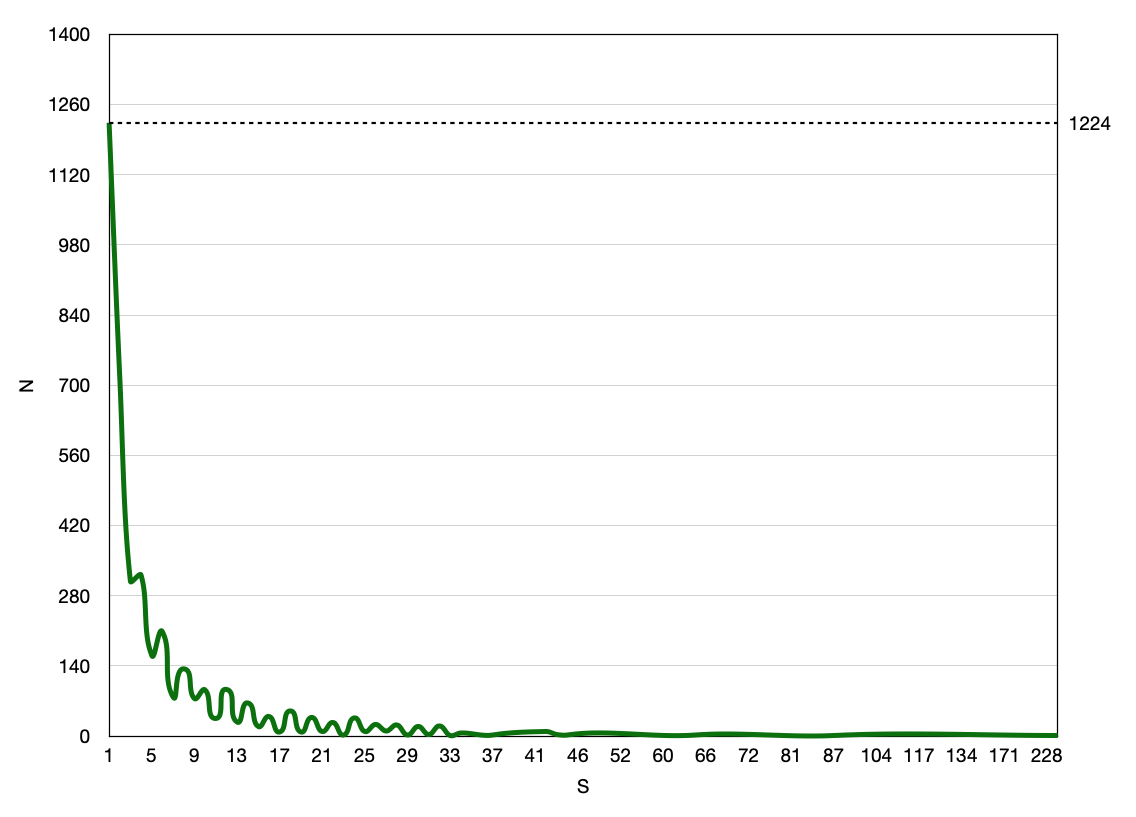
\includegraphics[width=\linewidth]{./chapter/city/Number_of_cities_having_given_number_of_sister_cities_according_to_Wikidata,_2020.png}}
}
  \caption{Зависимость числа городов (N) от числа имеющихся у этих городов побратимов (S), 2020 год.}
  \label{fig:city_relation_S_N}
\end{marginfigure}

\begin{itemize}
\item 32\% (\num{1314} городов) связаны братскими отношениями более чем с пятью городами;
\item 18\% (728 городов) имеют как минимум одиннадцать городов-побратимов;
\item 9\% (345 городов) подружились более чем с двадцатью городами;
\item 2\% (94 города) имеют от пятидесяти побратимов.
\end{itemize}

\begin{figure*}[h]
{
\setlength{\fboxsep}{0pt}%
\setlength{\fboxrule}{1pt}%
\fcolorbox{gray}{gray}{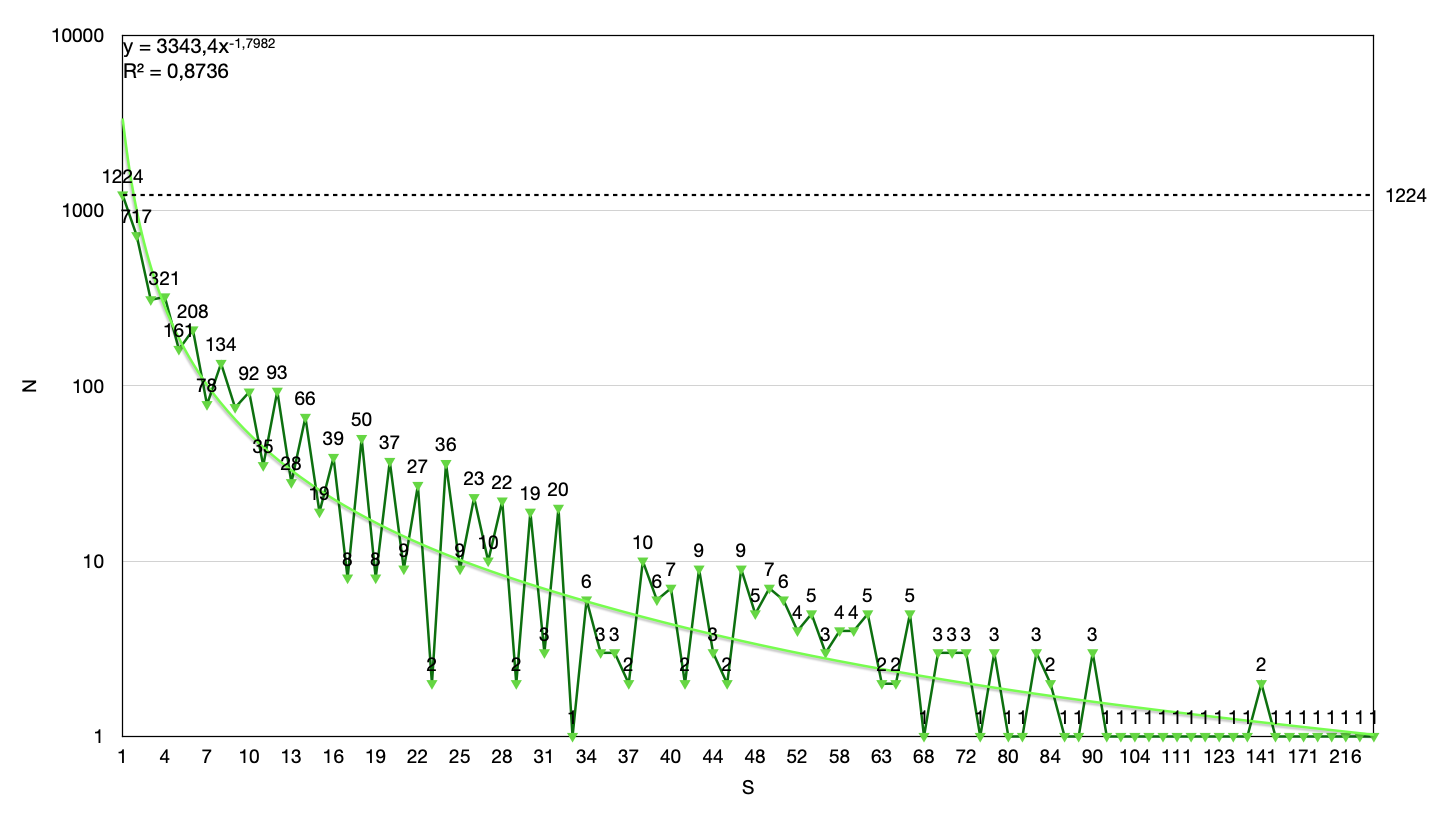
\includegraphics[width=\linewidth]{./chapter/city/Logarithm_of_the_number_of_cities_having_given_number_of_sister_cities_according_to_Wikidata,_2020.png}}%
}
  \caption{Логарифмическая зависимость числа городов (N) от числа имеющихся у этих городов побратимов (S), 2020 год.}%
  \label{fig:city_ln_relation_S_N}%
\end{figure*}

На основании построенного тренда можно сделать предположение, что зависимость числа городов от числа имеющихся у этих городов побратимов имеет распределение, близкое к степенному.

\begin{lstlisting}[ language=SPARQL, 
                    caption={\href{https://w.wiki/k7H}{Число городов России с определённым числом побратимов}\protect\footnotemark},
                    label=lst:city_relation_Russia_S_N, 
                    escapebegin=ку,escapeend=ку-ку>
                    ]
#defaultView:LineChart                                                   
# Count No. of cities having sisterCount sister cities  
# and number of sister cities themselves
SELECT ?sisterCount (COUNT(?sisterCount) AS ?FreqNSister) WHERE {                                                                                  
	{ # Count sister cities of cities which are ...
		SELECT (COUNT(?sister) AS ?sisterCount) WHERE {    
			{ ?city wdt:P31 wd:Q3957 } UNION # instances of "town"
			{ ?city wdt:P31 wd:Q515 } UNION # OR instances of "city"
			{ ?city wdt:P31 wd:Q1549591 } UNION # OR instances of "big city"
			{ ?city wdt:P31 wd:Q1637706 } # OR instances of "city 1000000+"
			?city wdt:P17 wd:Q159. # belonging to Russia
			?city wdt:P190 ?sister. # with filled property "sister city"
		}
		GROUP BY ?city # Group list by city                             
	}
}
GROUP BY ?sisterCount # Group by number of sister cities
ORDER BY DESC(?sisterCount) # Order by number of sister cities                                  
\end{lstlisting}
\footnotetext{Получено 24 варианта числа братских городов в 2020 году. Ссылка на SPARQL-запрос: \href{https://w.wiki/k7H}{https://w.wiki/k7H}}  

Ситуация с отечественными городами представлена на рис. \ref{fig:city_relation_Russia_S_N}. Чуть менее ста городов России (82 города) побратались хотя бы с одним городом, из них только 48\% (39 городов) связаны братскими отношениями более чем с пятью городами.

\begin{figure}
{
\setlength{\fboxsep}{0pt}%
\setlength{\fboxrule}{1pt}%
\fcolorbox{gray}{gray}{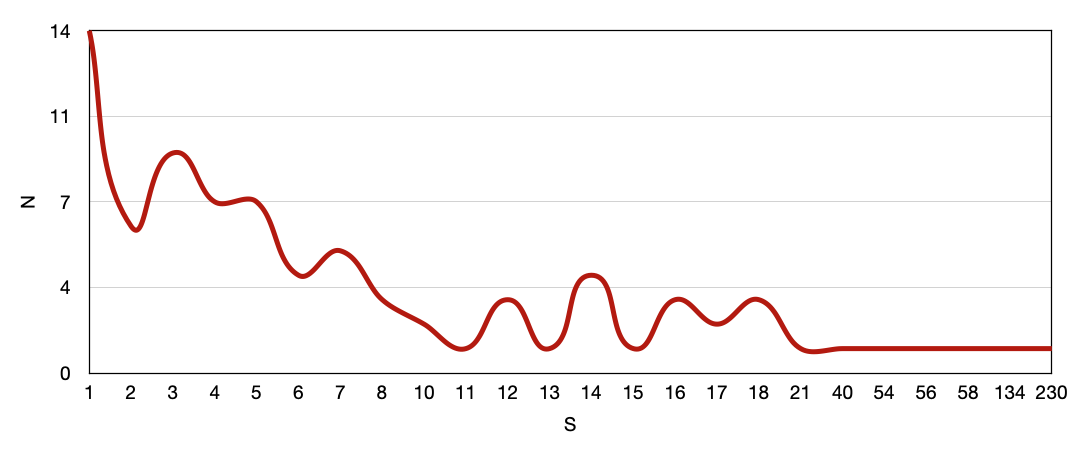
\includegraphics[width=\linewidth]{./chapter/city/Number_of_Russian_cities_having_given_number_of_sister_cities_according_to_Wikidata,_2020.png}}
}
  \caption{Зависимость числа городов России (N) от числа имеющихся у этих городов побратимов (S), 2020 год.}
  \label{fig:city_relation_Russia_S_N}
\end{figure}

\subsection{У какой страны больше всего побратимов?}

%%%%%%%%%%%%%%%% Упражнение 3 %%%%%%%%%%%%%%%%
\marginnote[-3.0cm]{
Какие из этих городов были основаны более 400 лет назад?
\begin{itemize}
\item \href{https://bit.ly/3lj8Jff}{Москва}
\item \href{https://bit.ly/3liUFSY}{Саров}
\item \href{https://bit.ly/38uwi11}{Казань}
\item \href{https://bit.ly/38r2dQ1}{Астрахань}
\item \href{https://bit.ly/3nhnEY1}{Самара}
\item \href{https://bit.ly/2GSNUZa}{Воронеж}
\end{itemize}
См. ответ~\ref{answer:cities_over_400_age} на с.~\pageref{answer:cities_over_400_age}.
}

Ниже представлен SPARQL-запрос для получения списка стран, упорядоченных по числу побратимов (листинг \ref{lst:countries_sister_cities}). Результаты данного запроса представлены на рис. \ref{fig:Bubble_countries_sister_cities}.

\begin{marginfigure}[0.5cm]
{
\setlength{\fboxsep}{0pt}%
\setlength{\fboxrule}{1pt}%
\fcolorbox{gray}{gray}{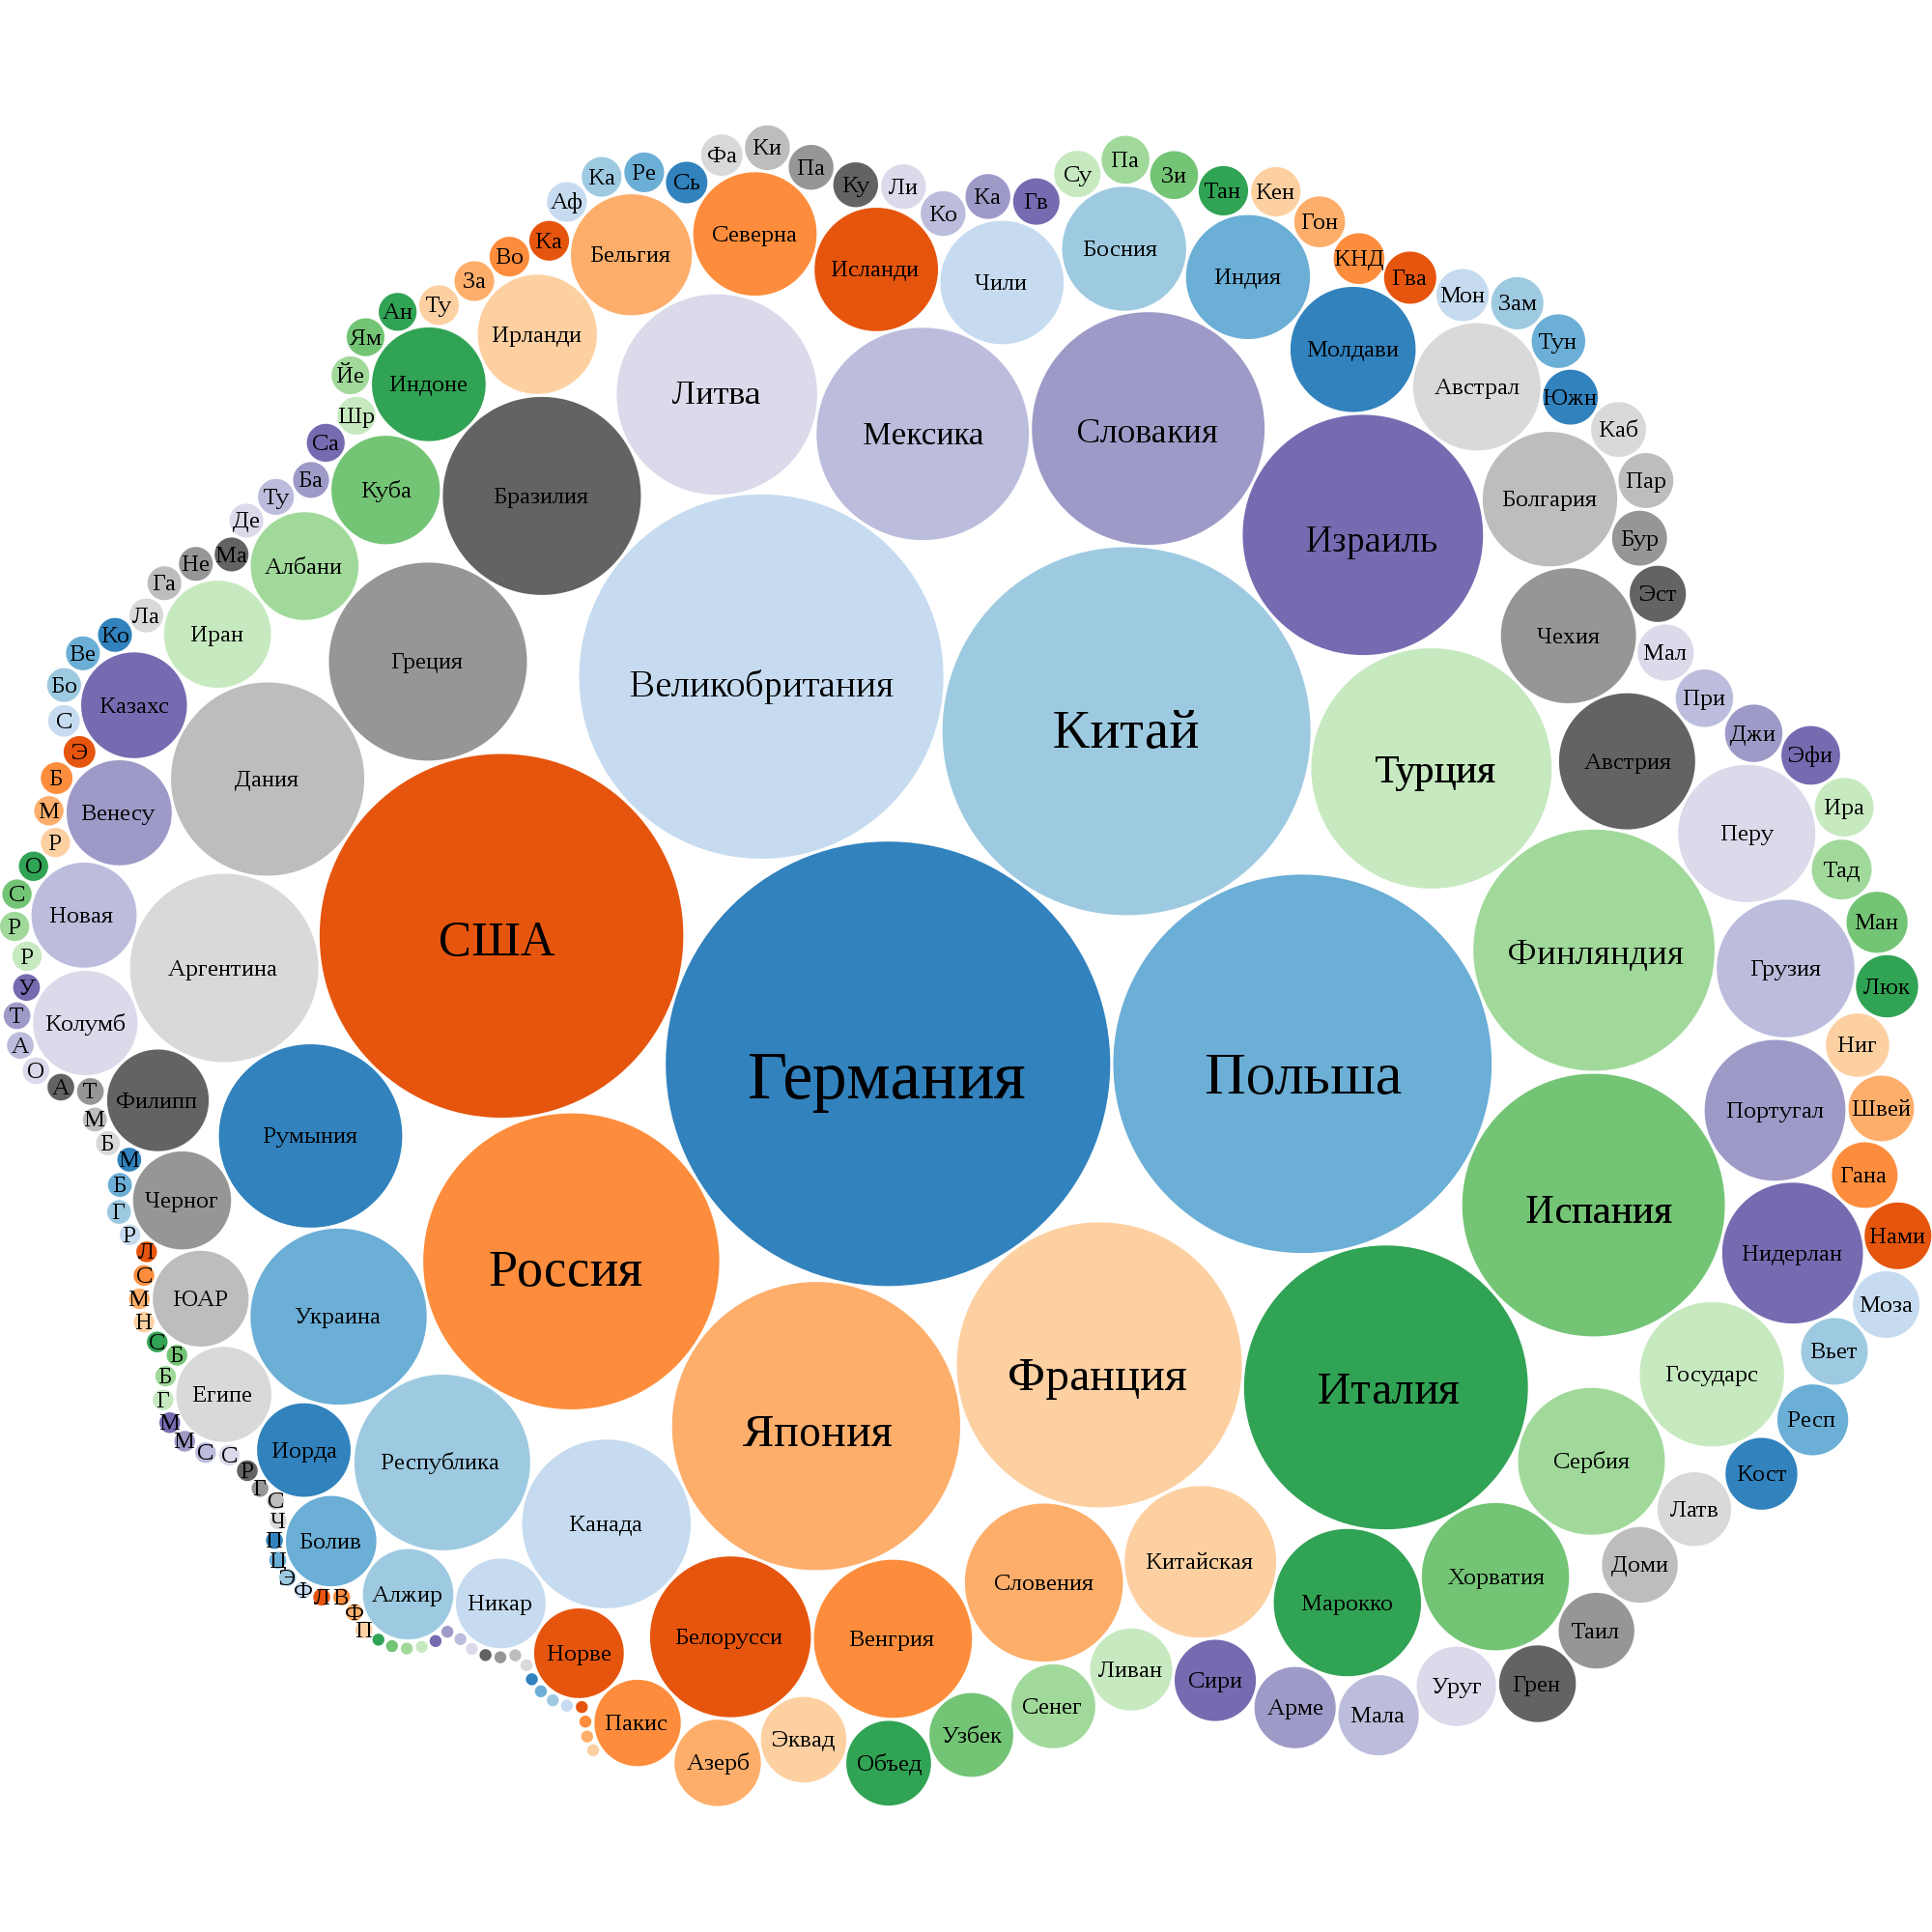
\includegraphics[width=\linewidth]{./chapter/city/Bubble_chart_number_of_sister_cities_of_countries_according_to_Wikidata,_2020_(RU).png}}%
}
  \caption{Пузырьковая диаграмма по числу побратимов у страны, 2020 год.}%
  \label{fig:Bubble_countries_sister_cities}%
\end{marginfigure}

\begin{lstlisting}[ language=SPARQL, 
                    caption={\href{https://w.wiki/k7R}{Упорядоченный список стран по числу побратимов}\protect\footnotemark},
                    label=lst:countries_sister_cities, 
                    escapebegin=ку,escapeend=ку-ку>
                    ]
#defaultView:BubbleChart
# Selecting number of distinct sister cities of particular country cities 
# which are ... 
SELECT ?countryLabel (COUNT(?sister) as ?sisterCount) WHERE { 
	SELECT DISTINCT ?countryLabel ?sister WHERE {
		{ ?city wdt:P31 wd:Q3957 } UNION # instances of "town"
		{ ?city wdt:P31 wd:Q515 } UNION # OR instances of "city"
		{ ?city wdt:P31 wd:Q1549591 } UNION # OR instances of "big city"
		{ ?city wdt:P31 wd:Q1637706 }.	 # OR instances of "city 1000000+"
		?city wdt:P17 ?country. # with filled property "country"
		?city wdt:P190 ?sister. # with filled property "sister city"
		SERVICE wikibase:label { bd:serviceParam wikibase:language "ru". }
	}                                 
}
GROUP BY ?countryLabel
ORDER BY DESC(?sisterCount)
\end{lstlisting}
\footnotetext{Получено 208 записей в 2020 году. Ссылка на SPARQL-запрос: \href{https://w.wiki/k7R}{https://w.wiki/k7R}}  

На 2020 год больше всего побратимов имела Германия (\num{1375} городов). В таблице~\ref{tab:germany_sister_cities} приведен список из 10 стран, имеющих наибольшее количество побратимов с городами Германии (2020). Получить полный список стран, с которыми Германия имеет города-побратимы, можно выполнив SPARQL-запрос, представленный ниже (листинг \ref{lst:sister_cities_with_Germany}).

\begin{table}
  \centering
  \fontfamily{ppl}\selectfont
  \begin{tabular}{| c | l | r | r |}
    \toprule
   \# & \multicolumn{1}{ c |}{Название страны} & \multicolumn{1}{p{0.3\textwidth} |}{\centering Количество городов-побратимов} & \multicolumn{1}{p{0.2\textwidth} |}{\centering \% от общего числа} \\
   \midrule
    1 & \wdqName{Франция}{142} & 247 & \num{18,0}\% \\
    2 & \wdqName{Германия}{183} & 195 & \num{14,2}\% \\
    3 & \wdqName{Великобритания}{145} & 120 & \num{8,7}\% \\
    4 & \wdqName{Италия}{38} & 86 & \num{6,3}\% \\
    5 & \wdqName{Польша}{36} & 81 & \num{5,9}\% \\
    6 & \wdqName{США}{30} & 60 & \num{4,4}\% \\
    7 & \wdqName{Австрия}{40} & 41 & \num{3,0}\% \\
    8 & \wdqName{Россия}{159} & 39 & \num{2,8}\% \\
    9 & \wdqName{Венгрия}{28} & 39 & \num{2,8}\% \\
    10 & \wdqName{Бельгия}{31} & 33 & \num{2,4}\% \\
    \bottomrule  \end{tabular}%
  \caption{Список стран, имеющих побратимы с городами Германии на 2020 год.}
  \label{tab:germany_sister_cities}
  %\zsavepos{pos:normaltab}
\end{table}

\begin{lstlisting}[ language=SPARQL, 
                    caption={\href{https://w.wiki/k7T}{Список стран, имеющих побратимы с городами Германии}\protect\footnotemark},
                    label=lst:sister_cities_with_Germany, 
                    escapebegin=ку,escapeend=ку-ку>
                    ]
# Selecting number of distinct particular country sister cities of cities 
# which are ...
SELECT ?country ?countryLabel 
				(COUNT(DISTINCT ?sister) as ?sisterCount) WHERE {                                                          
	{ ?city wdt:P31 wd:Q3957 } UNION # instances of "town"
	{ ?city wdt:P31 wd:Q515 } UNION # OR instances of "city"
	{ ?city wdt:P31 wd:Q1549591 } UNION # OR instances of "big city"      
	{ ?city wdt:P31 wd:Q1637706 }. # OR instances of "city 1000000+"
	?city wdt:P17 wd:Q183. # belonging to Germany  
	?city wdt:P190 ?sister. # with filled property "sister city" which are
	?sister wdt:P17 ?country. # with filled property "country"
	SERVICE wikibase:label { bd:serviceParam wikibase:language "ru". }
}
GROUP BY ?country ?countryLabel
ORDER BY DESC(?sisterCount)\end{lstlisting}
\footnotetext{Получено 93 записи в 2020 году. Ссылка на SPARQL-запрос: \href{https://w.wiki/k7T}{https://w.wiki/k7T}} 

\subsection{Ближайшие соседи России}

Ниже представлен SPARQL-запрос для получения списка стран, с которыми у России есть города-побратимы (листинг \ref{lst:countries_sister_cities_with_Russia}). Результаты данного запроса представлены на рис. \ref{fig:Bubble_countries_sister_cities_with_Russia}.

\begin{marginfigure}[0.0cm]
{
\setlength{\fboxsep}{0pt}%
\setlength{\fboxrule}{1pt}%
\fcolorbox{gray}{gray}{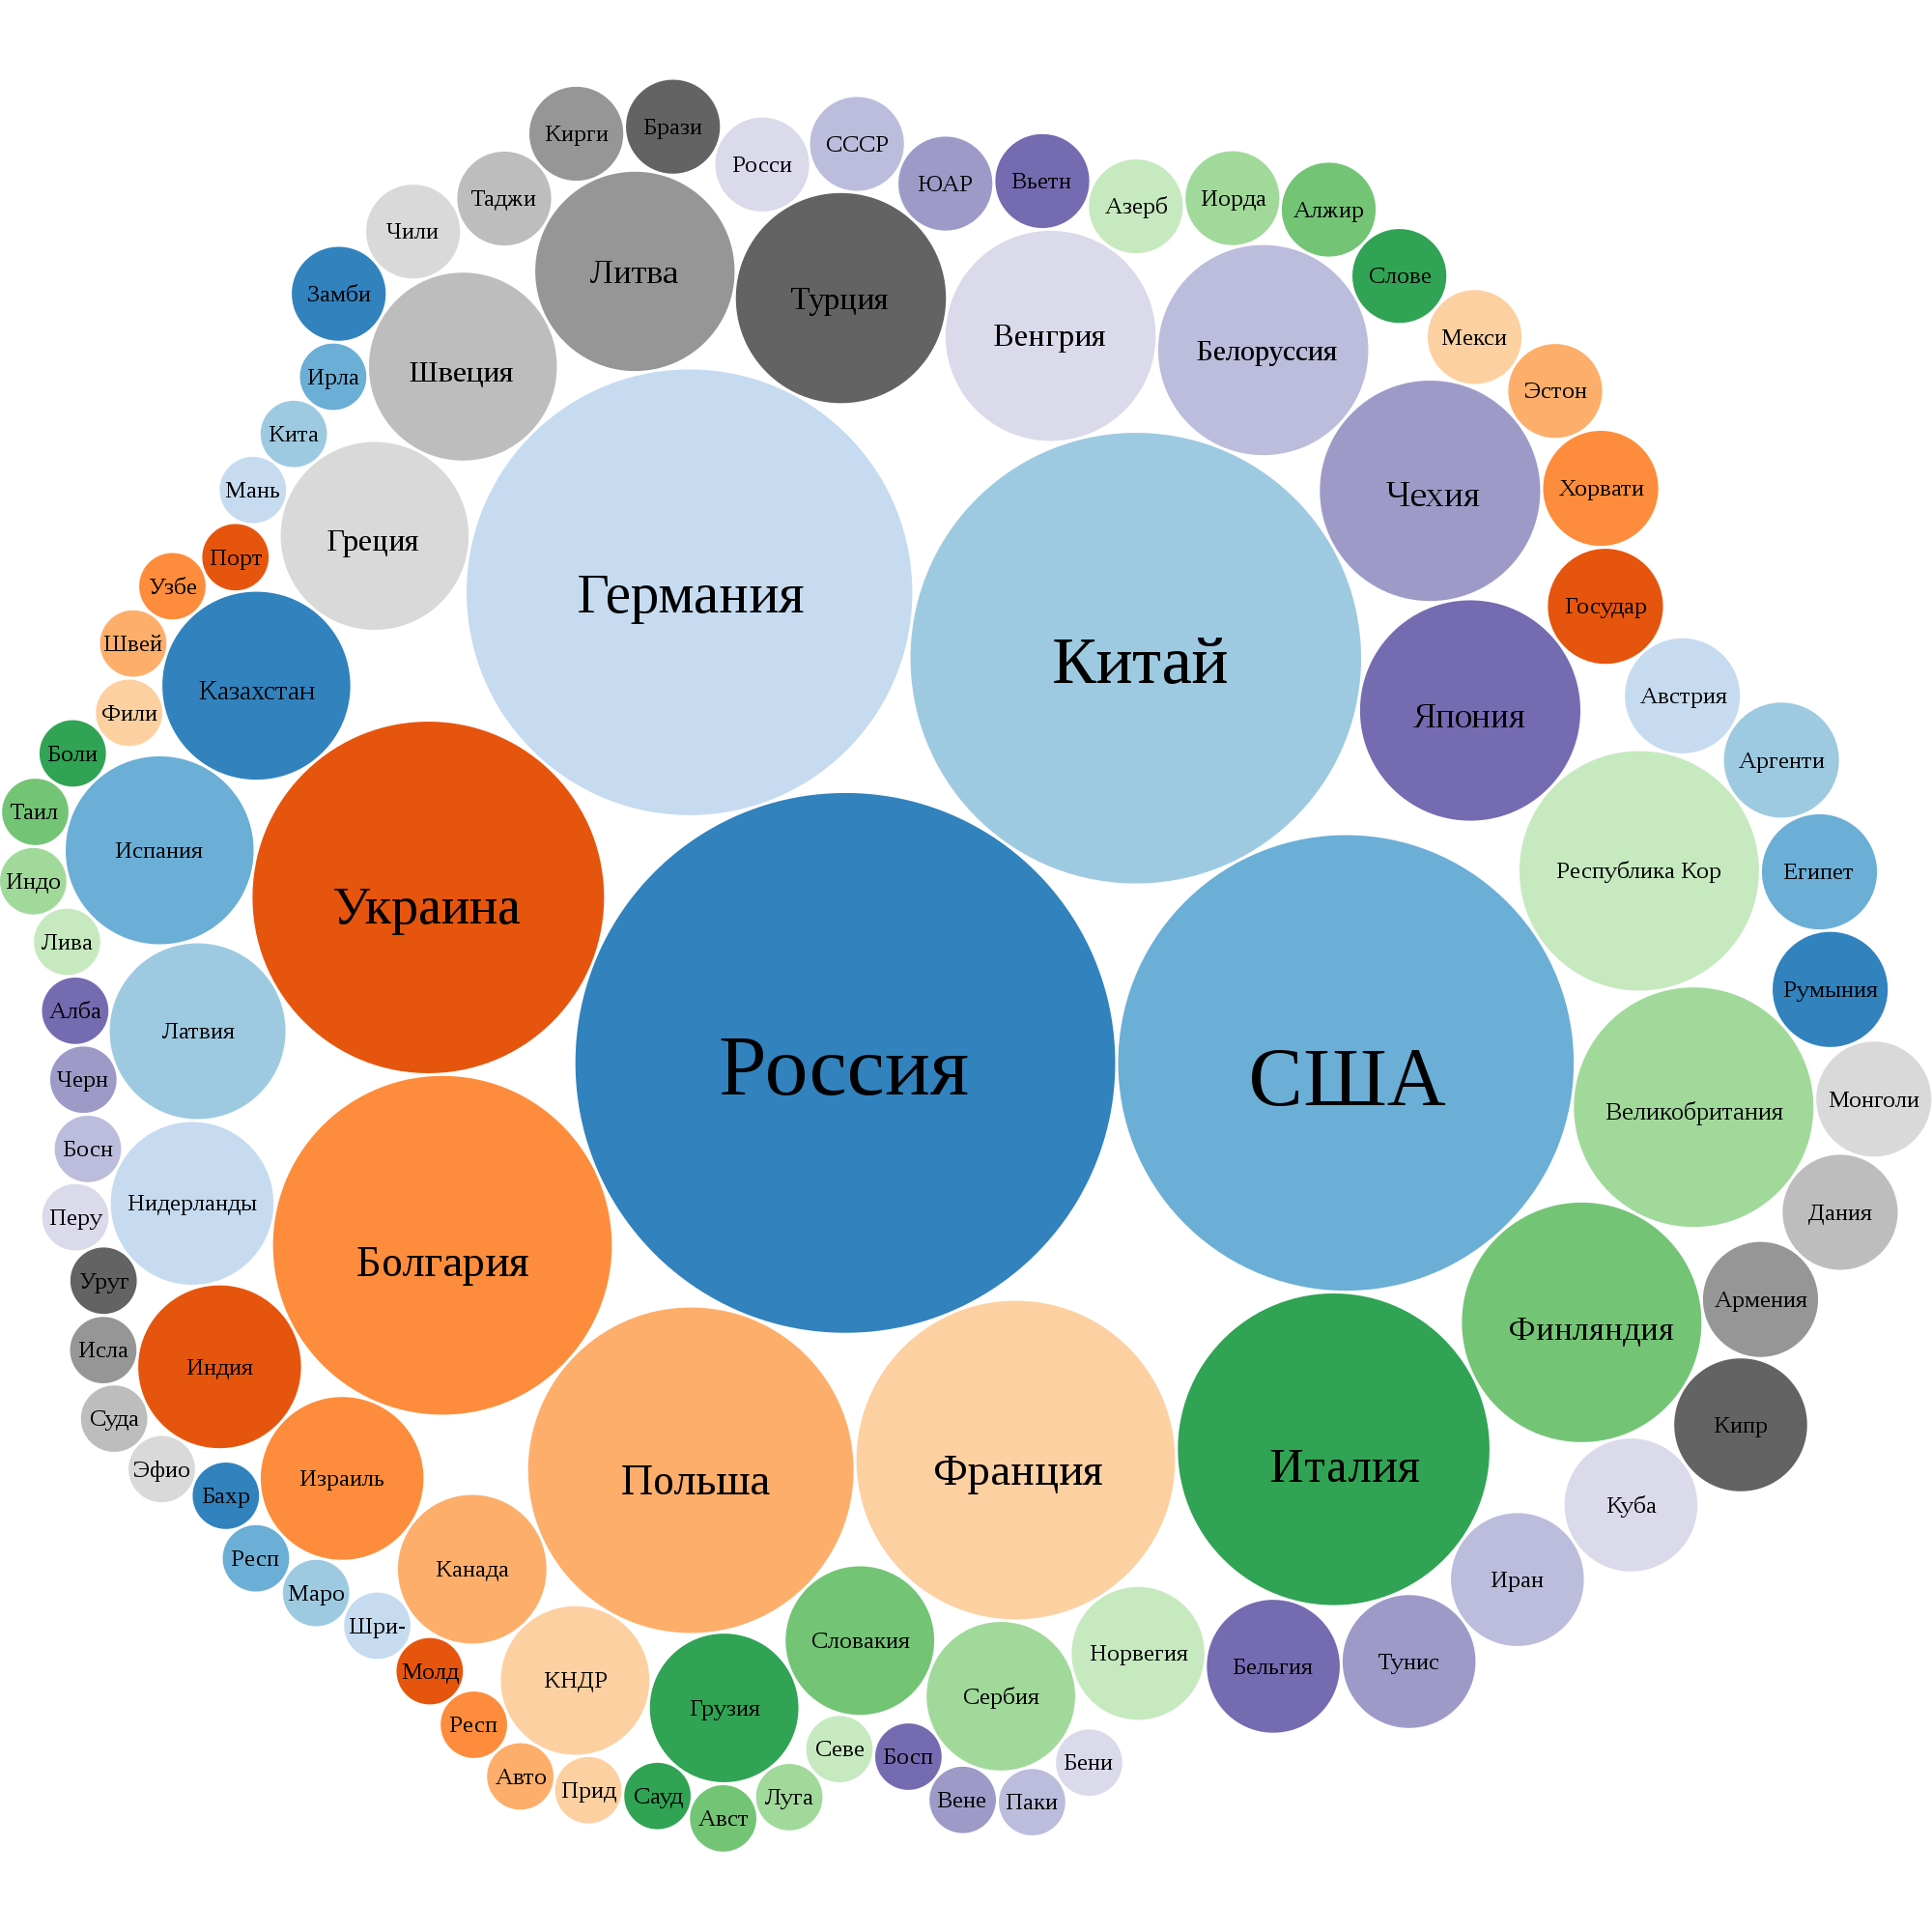
\includegraphics[width=\linewidth]{./chapter/city/Bubble_chart_number_of_sister_cities_with_Russia_of_countries_according_to_Wikidata,_2020_(RU).png}}%
}
  \caption{Пузырьковая диаграмма по числу побратимов у России со странами, 2020 год.}%
  \label{fig:Bubble_countries_sister_cities_with_Russia}%
\end{marginfigure}

\begin{lstlisting}[ language=SPARQL, 
                    caption={\href{https://w.wiki/k7W}{Ближайшие соседи России}\protect\footnotemark},
                    label=lst:countries_sister_cities_with_Russia, 
                    escapebegin=ку,escapeend=ку-ку>
                    ]
#defaultView:BubbleChart
# Selecting number of distinct particular country sister cities of cities 
# which are ...
SELECT ?country ?countryLabel 
				(COUNT(DISTINCT ?sister) as ?sisterCount) WHERE {                                                
	{ ?city wdt:P31 wd:Q3957 } UNION # instances of "town"
	{ ?city wdt:P31 wd:Q515 } UNION # OR instances of "city"
	{ ?city wdt:P31 wd:Q1549591 } UNION # OR instances of "big city"
	{ ?city wdt:P31 wd:Q1637706 }. # OR instances of "city 1000000+"                                 
	?city wdt:P17 wd:Q159. # belonging to Russia
	?city wdt:P190 ?sister. # with filled property "sister city" which are
	?sister wdt:P17 ?country. # with filled property "country"
	SERVICE wikibase:label { bd:serviceParam wikibase:language "ru". }
}
GROUP BY ?country ?countryLabel
ORDER BY DESC(?sisterCount)
\end{lstlisting}
\footnotetext{Получено 96 записей в 2020 году. Ссылка на SPARQL-запрос: \href{https://w.wiki/k7W}{https://w.wiki/k7W}}  

Больше двадцати городов-побратимов у России с такими странами, как США (47), Китай (46), Германия (45), Украина (28), Болгария (26), Польша (24), Франция (23) и Италия (22).

%%%%%%%%%%%%%%%%%%%%%%%%%%%%%%%%%%%%%%%%%%%%%%%%%%%%%%%
\section{Полнота и недостатки Викиданных}

%%%%%%%%%%%%%%%% Упражнение 2 %%%%%%%%%%%%%%%%
\marginnote{
Какому городу принадлежит флаг, изображенный на рис. \ref{fig:flag_question_city}?
}

\begin{marginfigure}[0.0cm]
{
\setlength{\fboxsep}{0pt}%
\setlength{\fboxrule}{1pt}%
\fcolorbox{gray}{gray}{
\includegraphics[width=\linewidth]{./chapter/city/Flag_of_Karabulak_(Ingushetia).png}}%
}
  \caption{Флаг одного из городов России.}%
  \label{fig:flag_question_city}%
\end{marginfigure}

\marginnote{
См. ответ~\ref{answer:cities_flags} на с.~\pageref{answer:cities_flags}.
}

Городом принято называть крупный населённый пункт, жители которого, как правило, не заняты сельским хозяйством. При этом разные страны используют различные критерии при наделении поселений статусом города, основным из которых является численность населения. Некоторые страны и вовсе не применяют понятие города. Так, во Франции используется только одна географическая единица подобного рода -- коммуна, вне зависимости от количества проживающих в ней людей и рода их деятельности. Поэтому чётко определить, какой населенный пункт относить к городам, а какой нет, может быть затруднительно.

На практике некоторые объекты Викиданных могут одновременно являться экземплярами городов разных типов. Например, \wdqName{Шанхай}{8686} отнесен к трем исследуемым объектам: \wdqName{city}{515}, \wdqName{big city}{1549591}, \wdqName{city with millions of inhabitants}{1637706}. Нетрудно догадаться, что такое множественное присваивание сказывается на результатах SPARQL-запросов, в частности, с использованием конструкции UNION. Это несложно проверить, выполнив, например, SPARQL-запрос по нахождению городов разных типов (линстинг \ref{lst:different_city_types}). \wdqName{Шанхай}{8686} встречается в результатах три раза. 

Викиданные имеют механизм наследования, выражающийся в свойстве \href{https://www.wikidata.org/wiki/Property:P279}{subclass of}. Заключается этот механизм в том, что если объект является экземпляром \wdqName{big city}{1549591}, то он является и экземпляром  \wdqName{city}{515}, так как \wdqName{big city}{1549591} -- подкласс  \wdqName{city}{515}. Таким образом, описанную выше ситуацию с \wdqName{Шанхаем}{8686} можно разрешить, оставив только один класс \wdqName{city with millions of inhabitants}{1637706}. Стоит отметить, что замена конструкции с использованием UNION (листинг \ref{lst:example_union_city}) на конструкцию с учетом подклассов неэквивалентна (листинг \ref{lst:example_subclasses_city}). Рассмотренный ранее \wdqName{Шанхай}{8686} встречается в новой выборке даже четыре раза. Дело в том, что помимо части исследуемых классов есть и другие наследуемые от \wdqName{city}{515}. Например, \wdqName{lost city}{2974842}, \wdqName{free imperial city}{57318}, \wdqName{autonomous city}{1094397} и даже \wdqName{ideal city}{1656724}.

\begin{lstlisting}[ language=SPARQL, 
                    caption={\href{https://w.wiki/k5T}{Пример использования конструкции UNION}\protect\footnotemark},
                    label=lst:example_union_city, 
                    escapebegin=ку,escapeend=ку-ку>
                    ]
SELECT ?city ?cityLabel WHERE { # Selecting items which are ...
	{ ?city wdt:P31 wd:Q515 } UNION # instances of "city"            
	{ ?city wdt:P31 wd:Q1549591 } UNION # instances of "big city"               
	{ ?city wdt:P31 wd:Q1637706 } 	# instances of "city 1000000+"
	SERVICE wikibase:label { bd:serviceParam wikibase:language "ru". }
}
\end{lstlisting}
\footnotetext{Ссылка на SPARQL-запрос: \href{https://w.wiki/k5T}{https://w.wiki/k5T}}

\begin{lstlisting}[ language=SPARQL, 
                    caption={\href{https://w.wiki/jyB}{Пример использования конструкции с подклассами}\protect\footnotemark},
                    label=lst:example_subclasses_city, 
                    escapebegin=ку,escapeend=ку-ку>
                    ]
SELECT ?city ?cityLabel WHERE { # Selecting items which are ...
	?city wdt:P31/wdt:P279* wd:Q515 # instances of "city" subclasses
	SERVICE wikibase:label { bd:serviceParam wikibase:language "ru". }
}
\end{lstlisting}
\footnotetext{Ссылка на SPARQL-запрос: \href{https://w.wiki/jyB}{https://w.wiki/jyB}}

Также, вероятно с неоднозначностью критериев присвоения статуса города, были созданы подклассы для конкретных стран -- \wdqName{city in Chile}{25412763}, \wdqName{city in Cyprus}{29556224}, \wdqName{city of Japan}{494721} и так далее. Не обошла стороной эта тенденция и города России, что можно было заметить при сравнении результатов SPARQL-запроса для нахождения экземпляров объекта <<город>> (листинг \ref{lst:city}). На данный момент большинство из них принадлежат классу \wdqName{city/town}{7930989}.

По данным \href{http://www.gks.ru/free\_doc/new\_site/perepis2010/croc/Documents/Vol1/pub-01-03.pdf}{всероссийской переписи населения (2010)}\cite{city_perepis_2010} и \href{https://rosstat.gov.ru/free\_doc/new\_site/population/demo/perepis\_krim/KRUM\_2015.pdf}{переписи населения в Крымском федеральном округе (2014)}\cite{city_perepis_2014} суммарное число городов России составило \num{1117} на 2014 год. Все \href{https://bit.ly/32yqpw5}{города России} имеют страницу как в русской, так и в английской Википедии.

Число элементов Викиданных, являющихся российскими городами -- \href{https://w.wiki/jyP}{1126} . Можно предположить, что Викиданные полностью покрывают, как минимум, российские города. 

%%%%%%%%%%%%%%%%%%%%%%%%%%%%%%%%%%%%%%%%%%%%%%%%%%%%%%%
\section{Упражнения}
\begin{enumerate}
\item Построить граф братских городов России.
\item Получить список городов России, находящихся за полярным кругом.
\item На какой реке в России стоит наибольшее число городов?
\end{enumerate}